\documentclass[aspectratio=169]{beamer}
\usetheme{Boadilla}
\usecolortheme{default}
\usefonttheme{default}

\usepackage[T1]{fontenc}
\usepackage[utf8]{inputenc}
\usepackage{lmodern}
\usepackage{amsmath}
\usepackage{booktabs}
\usepackage{graphicx}
\usepackage{listings}
\usepackage{xcolor}

\title{Control Variates for a GARCH Model}
\subtitle{Monte Carlo Project -- Oral Support}
\author[A. Bernabeu, T. Bourdareau, N. Grimaldi]{Adam BERNABEU, Tom BOURDAREAU, Nicolas GRIMALDI}
\date{\today}

\lstdefinestyle{py}{
  language=Python,
  basicstyle=\ttfamily\tiny,
  keywordstyle=\color{blue!70!black},
  commentstyle=\color{green!40!black},
  stringstyle=\color{orange!60!black},
  showstringspaces=false,
  breaklines=true,
  frame=single
}

\begin{document}

\begin{frame}
	\titlepage
\end{frame}

\begin{frame}{Part 0 -- Article Presentation}
	\textbf{Reference paper:}
	\begin{itemize}
		\item MCMC for GARCH posterior inference with variance reduction ideas.
		\item Main tool: \textbf{control variates} to reduce Monte Carlo error.
		\item Our implementation follows the experiment protocol:
		      \begin{itemize}
			      \item Random Walk Metropolis for a GARCH(1,1) posterior.
			      \item Comparison of estimators (plain MCMC vs corrected estimators).
		      \end{itemize}
		\item Second paper extends to high-dimensional control variates via Lasso.
	\end{itemize}
\end{frame}

\begin{frame}{Part 1 -- Question 1}
	\Large
	\textbf{Implement a Random Walk Metropolis sampler}\\[0.4em]
	for a GARCH(1,1) posterior, first on simulated data,\\[0.2em]
	then on real exchange-rate log-returns.
\end{frame}

\begin{frame}{Q1 -- Mathematical setup}
	\small
	\[
		r_t = \sqrt{h_t}\,\varepsilon_t,\qquad \varepsilon_t \sim \mathcal N(0,1),
	\]
	\[
		h_t = \omega_1 + \omega_2 r_{t-1}^2 + \omega_3 h_{t-1},
		\quad \omega_1>0,\ \omega_2,\omega_3\ge 0,\ \omega_2+\omega_3<1.
	\]
	\[
		\pi(\omega \mid r_{1:T}) \propto L(r_{1:T}\mid \omega)\,p(\omega).
	\]
	\[
		\alpha(\omega,\omega')=\min\!\left(
		1,\frac{\pi(\omega' \mid r)}{\pi(\omega \mid r)}
		\right).
	\]
	\begin{itemize}
		\item Random-walk proposal: \(\omega'=\omega+\eta,\ \eta\sim\mathcal N(0,\Sigma)\).
	\end{itemize}
\end{frame}

\begin{frame}[fragile]{Q1 -- Data visualisation}
	\begin{columns}[T,totalwidth=\textwidth]
		\column{0.5\textwidth}
		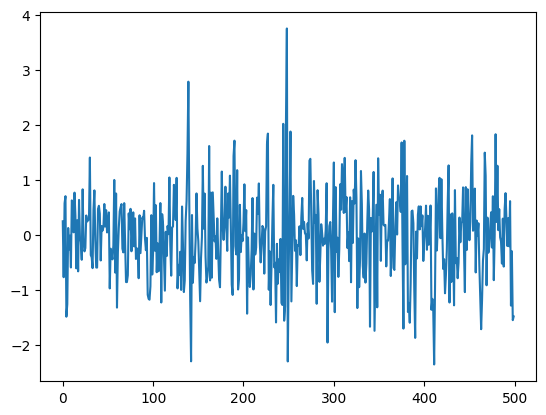
\includegraphics[width=\linewidth,height=0.62\textheight,keepaspectratio]{assets/notebook/simu_graph.png}
		\column{0.5\textwidth}
		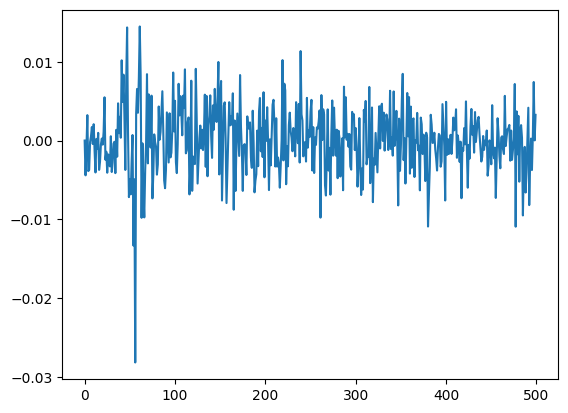
\includegraphics[width=\linewidth,height=0.62\textheight,keepaspectratio]{assets/notebook/real_graph.png}
	\end{columns}
	\begin{itemize}
		\item On the left the simulation, on the right the real data from EUR/USD.
	\end{itemize}

\end{frame}

\begin{frame}[fragile]{Q1 -- Core sampler (code extract)}
	\begin{lstlisting}[style=py]
def metropolis_hastings(r, iters=10000, scale=1.0):
    chain = np.zeros((iters, 3))
    current_w = np.array([0.1, 0.1, 0.7])
    current_ll = log_likelihood(current_w, r)
    current_lp = log_prior(current_w)
    for i in range(iters):
        proposal_w = current_w + rng.normal(0, step_sizes, 3)
        proposal_lp = log_prior(proposal_w)
        if proposal_lp > -np.inf:
            proposal_ll = log_likelihood(proposal_w, r)
            log_ratio = (proposal_ll + proposal_lp) - (current_ll + current_lp)
            if np.log(rng.random()) < log_ratio:
                current_w = proposal_w
                current_ll = proposal_ll
                current_lp = proposal_lp
        chain[i] = current_w
\end{lstlisting}
	\vspace{-0.5em}
	\begin{itemize}
		\item Prior constraints enforce positivity and stationarity ($\omega_2+\omega_3<1$).
	\end{itemize}
\end{frame}

\begin{frame}{Q1 -- Simulated-data diagnostics}
	\begin{columns}[T,totalwidth=\textwidth]
		\column{0.5\textwidth}
		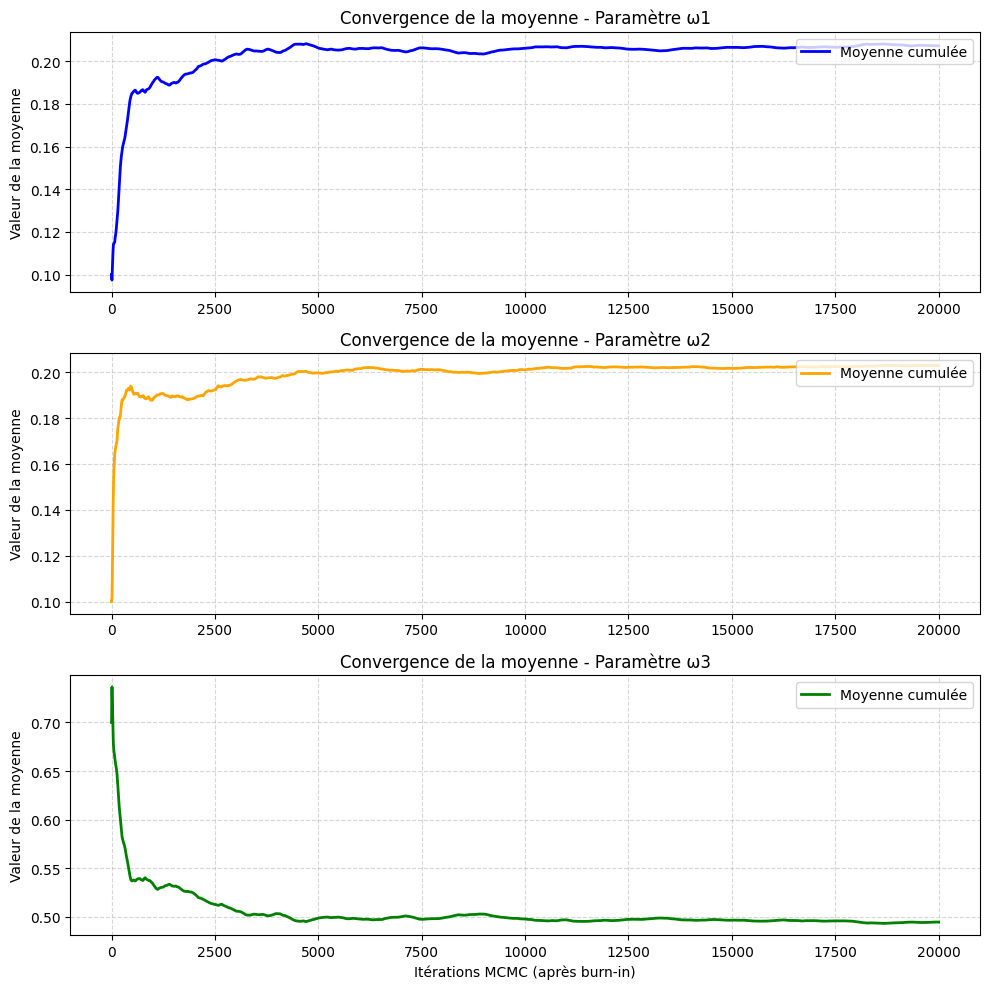
\includegraphics[width=\linewidth,height=0.62\textheight,keepaspectratio]{assets/notebook/q1_cell_11_out_00.png}
		\column{0.5\textwidth}
		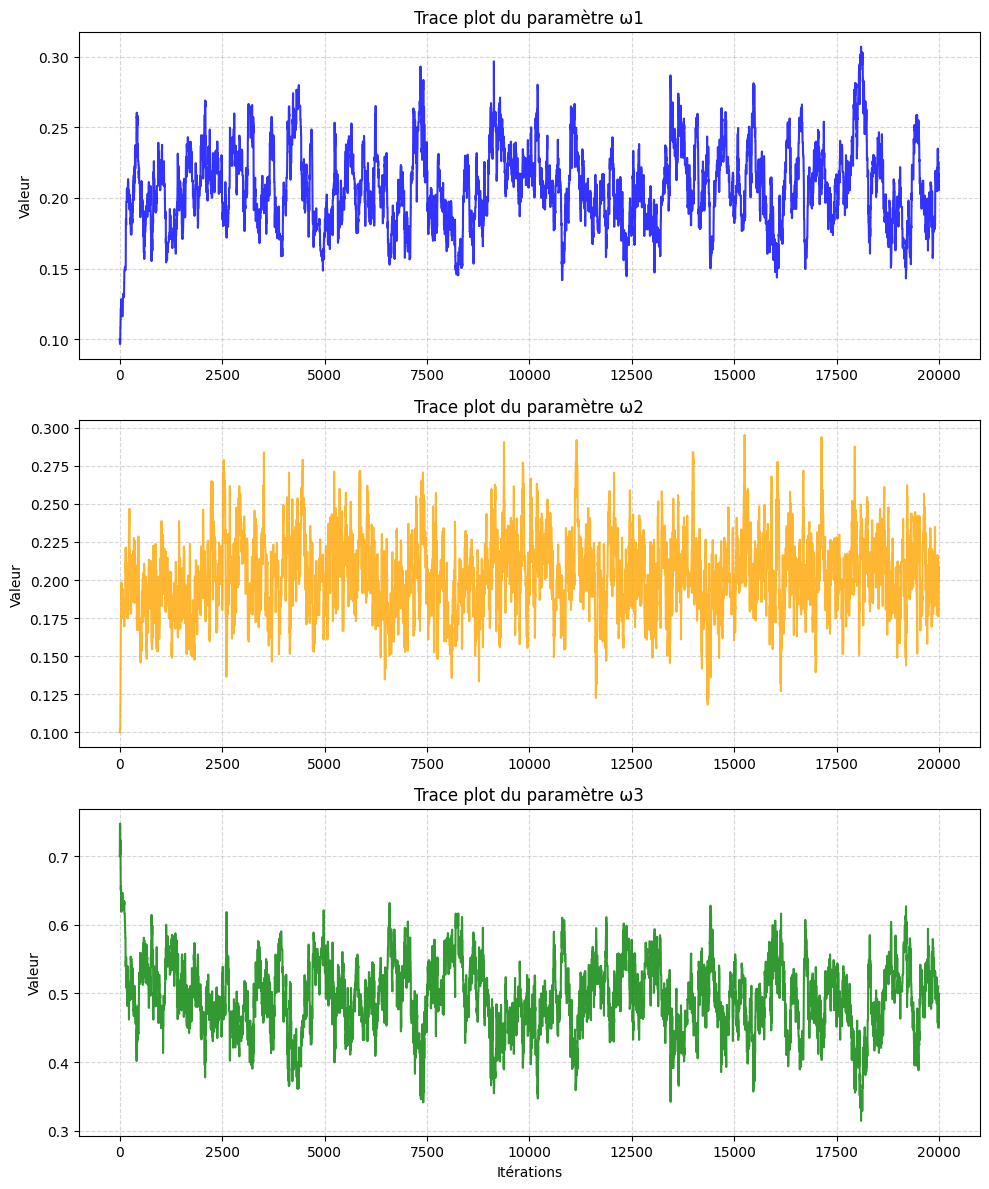
\includegraphics[width=\linewidth,height=0.62\textheight,keepaspectratio]{assets/notebook/q1_cell_12_out_00.png}
	\end{columns}
	\begin{itemize}
		\item Trace plots stabilize after burn-in with the tuned proposal scale.
	\end{itemize}
\end{frame}

\begin{frame}{Q1 -- Posterior distributions and repeatability}
	\begin{columns}[T,totalwidth=\textwidth]
		\column{0.5\textwidth}
		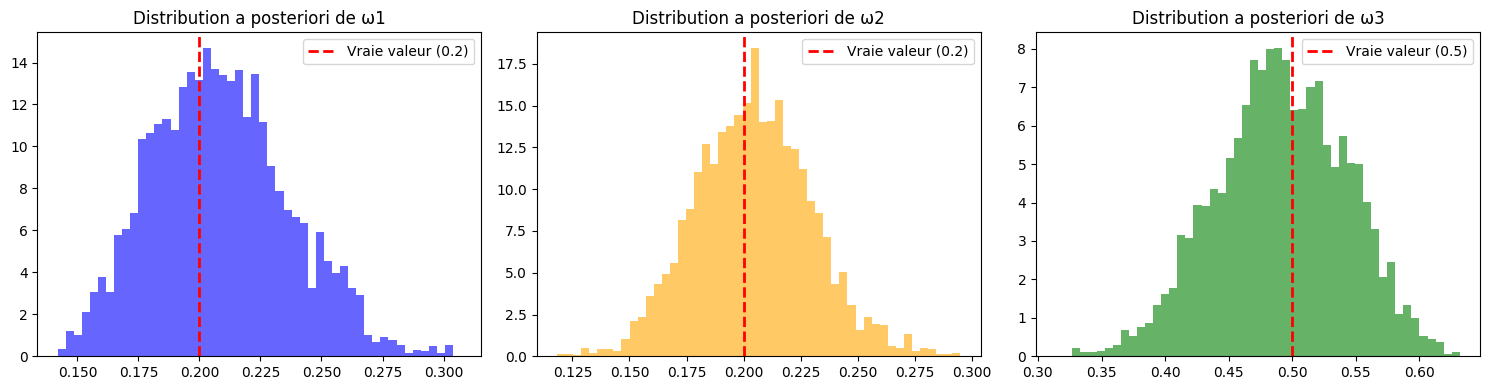
\includegraphics[width=\linewidth]{assets/notebook/q1_cell_13_out_00.png}
		\column{0.5\textwidth}
		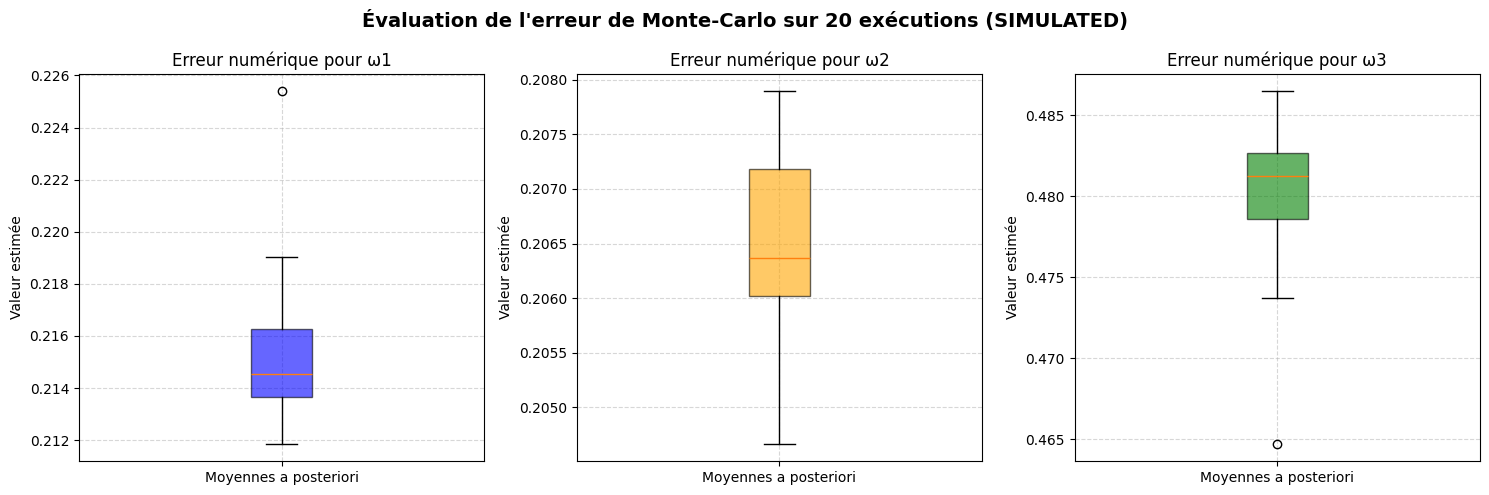
\includegraphics[width=\linewidth]{assets/notebook/q1_cell_23_out_00.png}
	\end{columns}
	\vspace{0.2em}
	\begin{itemize}
		\item Repeated runs show visible Monte Carlo variability.
		\item This motivates control variates in Q2--Q3.
	\end{itemize}
\end{frame}

\begin{frame}{Q1 -- Real-data run (EUR/USD log-returns)}
	\begin{columns}[T,totalwidth=\textwidth]
		\column{0.333\textwidth}
		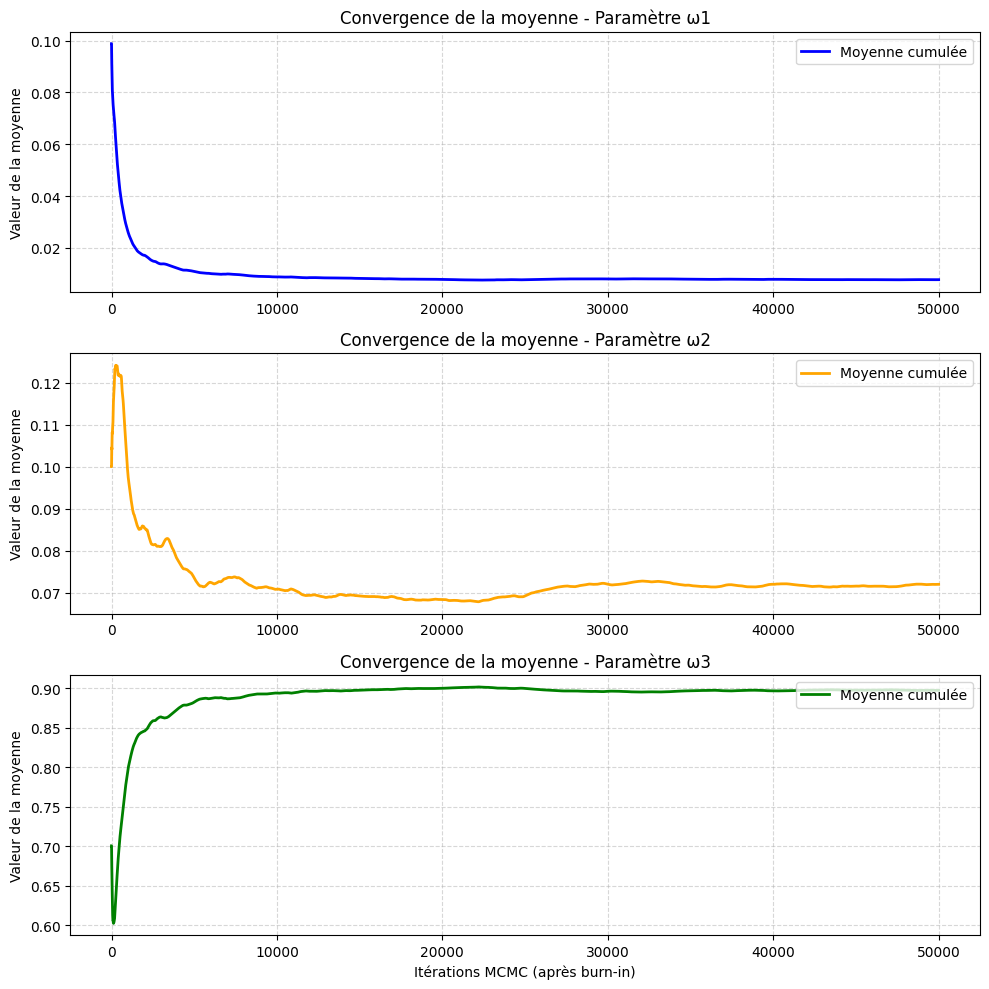
\includegraphics[width=\linewidth]{assets/notebook/q1_cell_17_out_00.png}
		\column{0.333\textwidth}
		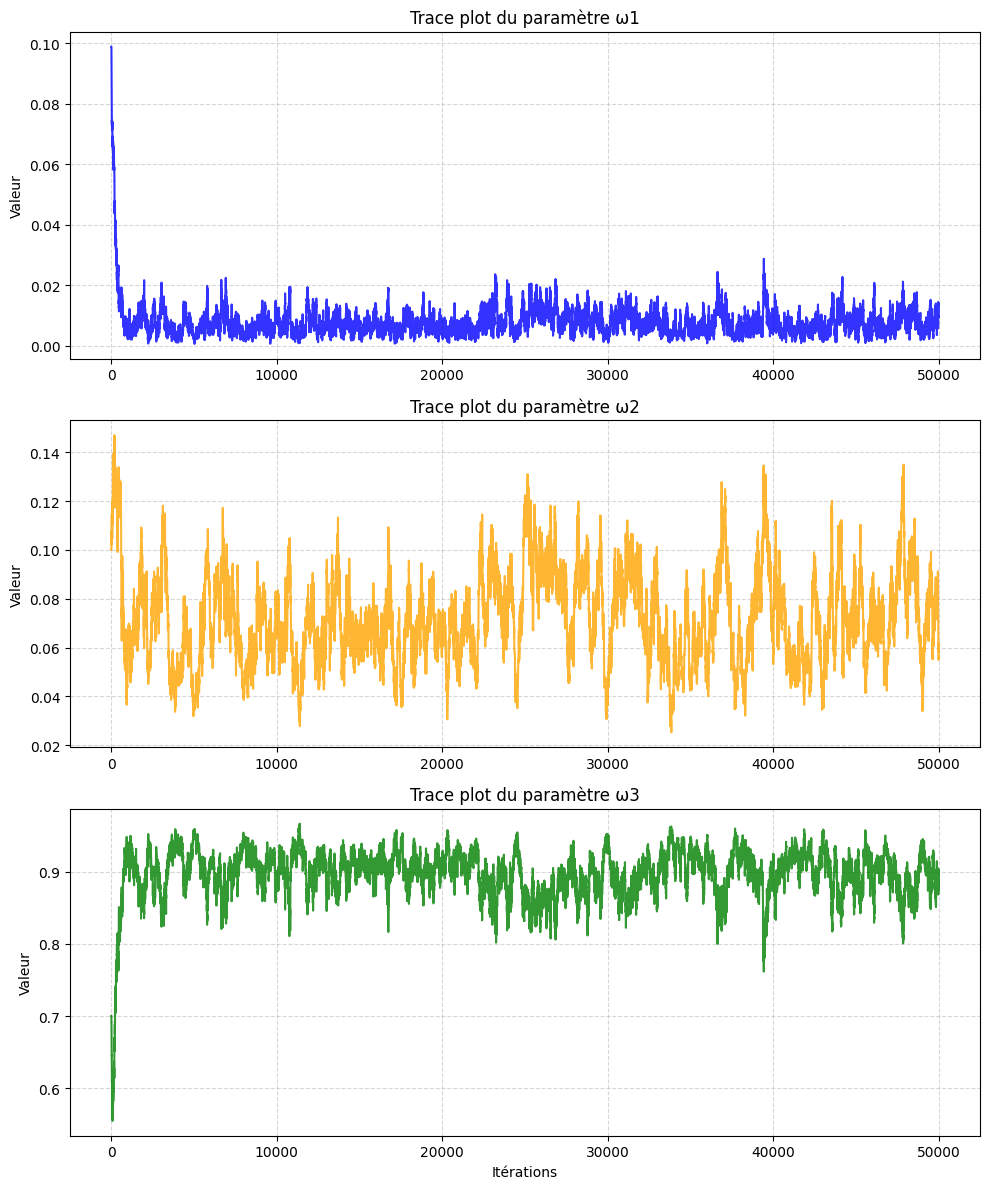
\includegraphics[width=\linewidth]{assets/notebook/q1_cell_18_out_00.png}
		\column{0.333\textwidth}
		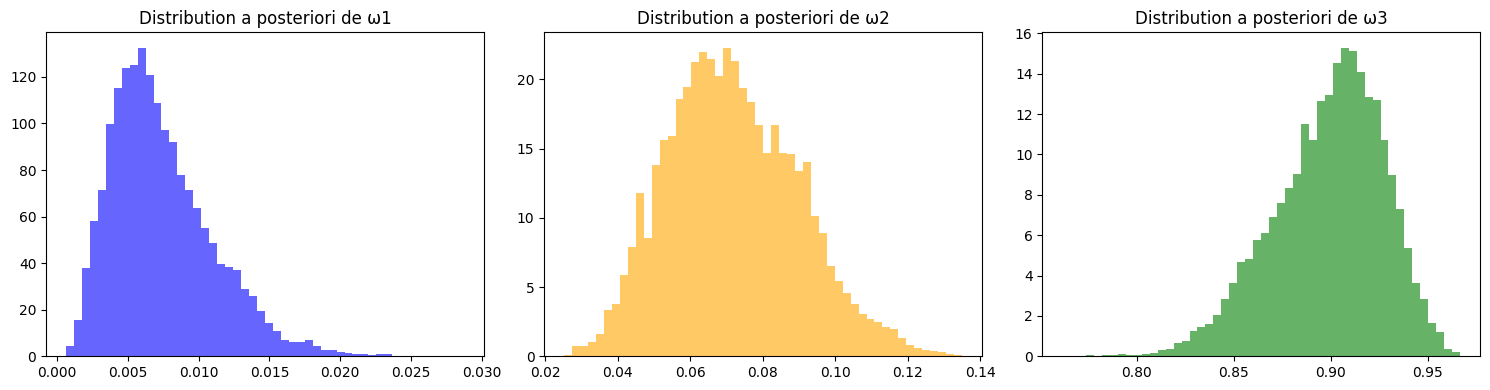
\includegraphics[width=\linewidth]{assets/notebook/q1_cell_19_out_00.png}
	\end{columns}
	\vspace{0.2em}
	\begin{itemize}
		\item Same pipeline transfers to market data.
		\item Real data confirms the need for variance reduction.
	\end{itemize}
\end{frame}

\begin{frame}{Part 2 -- Question 2}
	\Large
	\textbf{Use first-order control variates}\\[0.4em]
	and estimate coefficients by linear regression\\[0.2em]
	to reduce estimator variance.
\end{frame}

\begin{frame}{Q2 -- Math for degree-1 control variates}
	\small
	Target quantity:
	\[
		\mu_f=\mathbb E_{\pi}[f(\omega)].
	\]
	First-order corrected estimator:
	\[
		\tilde f(\omega)=f(\omega)+a^\top z(\omega),
		\qquad
		z(\omega)\approx -\tfrac12\nabla \log \pi(\omega\mid r).
	\]
	Choose \(a\) by regression over MCMC samples:
	\[
		f(\omega^{(i)})=\beta_0 + b^\top z(\omega^{(i)})+\varepsilon_i,
		\quad a=-b.
	\]
	\[
		\hat\mu_f^{\,cv}=\frac1N\sum_{i=1}^N \tilde f(\omega^{(i)}).
	\]
\end{frame}

\begin{frame}[fragile]{Q2 -- First-order ZV control variates}
	\begin{lstlisting}[style=py]
@njit
def compute_garch_gradient_fast(w, r):
    # returns Z(w) = -0.5 * grad log pi(w)
    ...

# Regression correction for each target function f
X = Z_run
Y = f_samples
reg = LinearRegression().fit(X, Y)
f_corrected = Y - X @ reg.coef_
\end{lstlisting}
	\vspace{-0.5em}
	\begin{itemize}
		\item Linear model gives the best coefficients in least-squares sense.
		\item Cost is moderate for degree-1 features.
	\end{itemize}
\end{frame}

\begin{frame}{Q2 -- Variance reduction results}
	\begin{columns}[T,totalwidth=\textwidth]
		\column{0.5\textwidth}
		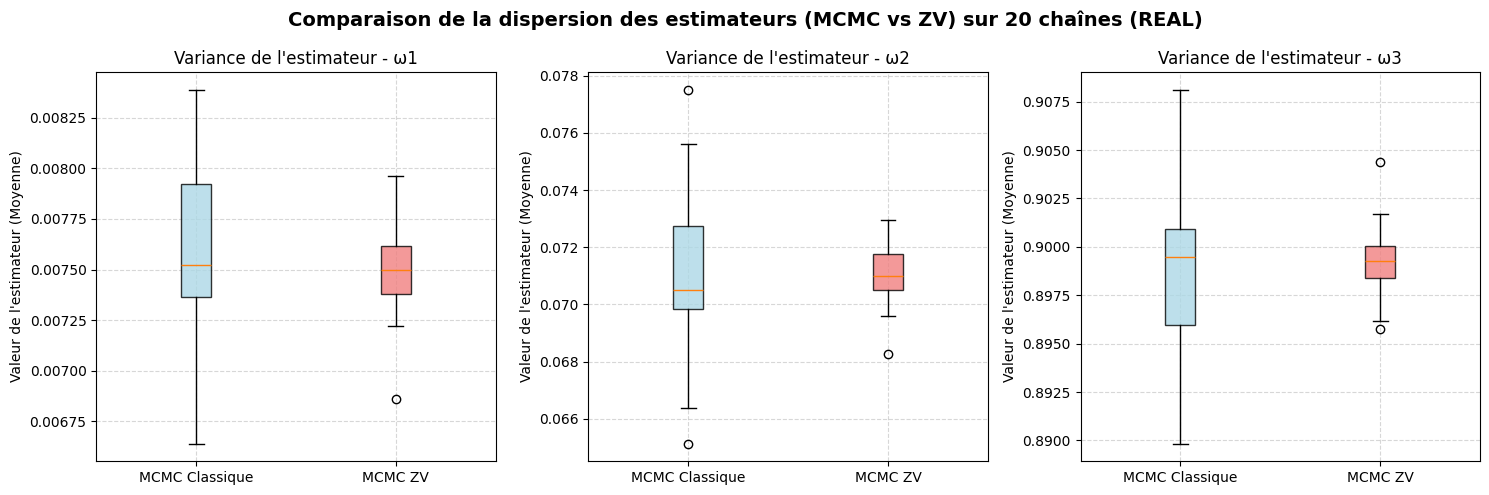
\includegraphics[width=\linewidth]{assets/notebook/q2_cell_27_out_00.png}
		\column{0.5\textwidth}
		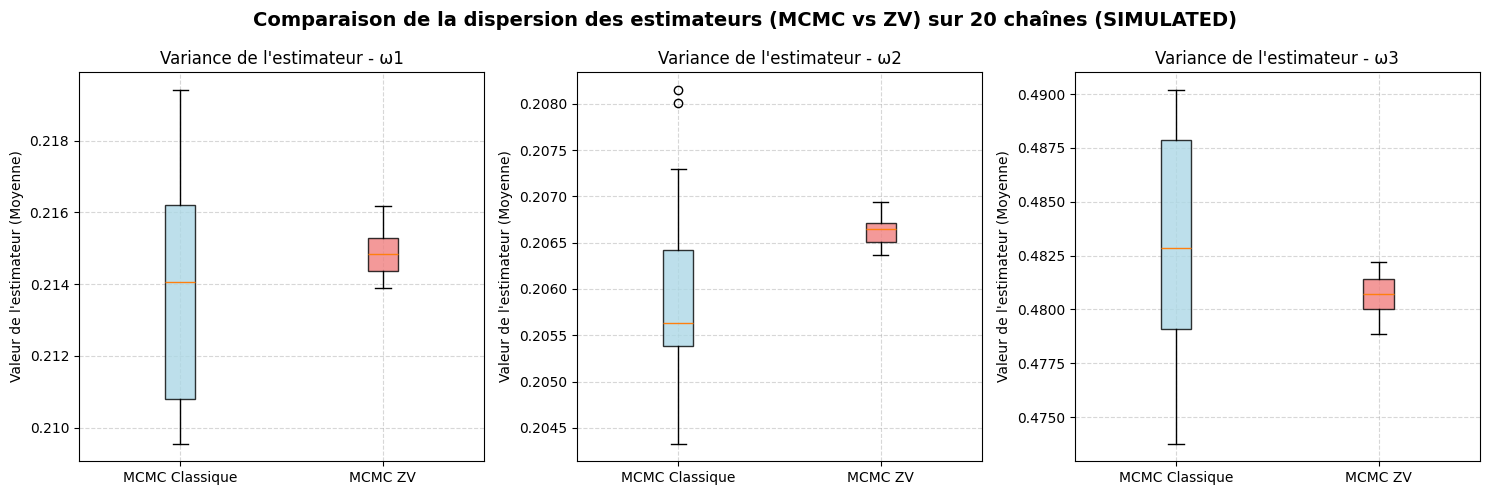
\includegraphics[width=\linewidth]{assets/notebook/q2_cell_28_out_00.png}
	\end{columns}
	\vspace{0.2em}
	\begin{itemize}
		\item Boxplots show narrower dispersion than naive MCMC means.
		\item Numerical-error assessment is done over repeated runs.
	\end{itemize}
\end{frame}

\begin{frame}{Part 3 -- Question 3}
	\Large
	\textbf{Use a larger set of control variates (degree 2),}\\[0.4em]
	then adapt the Lasso-based approach\\[0.2em]
	to handle feature explosion.
\end{frame}

\begin{frame}{Q3 -- Degree-2 controls and Lasso}
	\small
	Degree-2 basis (schematically):
	\[
		\phi(\omega)=\big[z_1,z_2,z_3,\ \omega_j z_i-\delta_{ij}/2\big]_{i,j=1}^3
		\in \mathbb R^{12}.
	\]
	High-dimensional issue (for larger models):
	\[
		p \uparrow \Rightarrow X^\top X \text{ inversion unstable/costly}.
	\]
	Lasso correction:
	\[
		\hat\beta=\arg\min_{\beta}
		\frac{1}{2N}\|y-X\beta\|_2^2+\lambda\|\beta\|_1,
	\]
	\[
		\hat\mu_f^{\,lasso}=\frac1N\sum_{i=1}^N\left(f_i-(X\hat\beta)_i\right).
	\]
\end{frame}

\begin{frame}[fragile]{Q3 -- Why Lasso? (code extract)}
	\begin{lstlisting}[style=py]
# Degree-2 design: 3 first-order + 9 second-order terms
features = []
for i in range(3):
    features.append(Z_run[:, i])
for i in range(3):
    for j in range(3):
        delta = 0.5 if i == j else 0.0
        features.append(W_run[:, j] * Z_run[:, i] - delta)
X_design = np.column_stack(features)

lasso = LassoCV(cv=5).fit(X_design, Y)
Y_corr = Y - X_design @ lasso.coef_
\end{lstlisting}
	\vspace{-0.5em}
	\begin{itemize}
		\item Feature count grows quickly with polynomial order.
		\item Lasso keeps only useful controls and stabilizes estimation.
	\end{itemize}
\end{frame}

\begin{frame}{Q3 -- LSLASSO vs naive regression}
	\begin{columns}[T,totalwidth=\textwidth]
		\column{0.5\textwidth}
		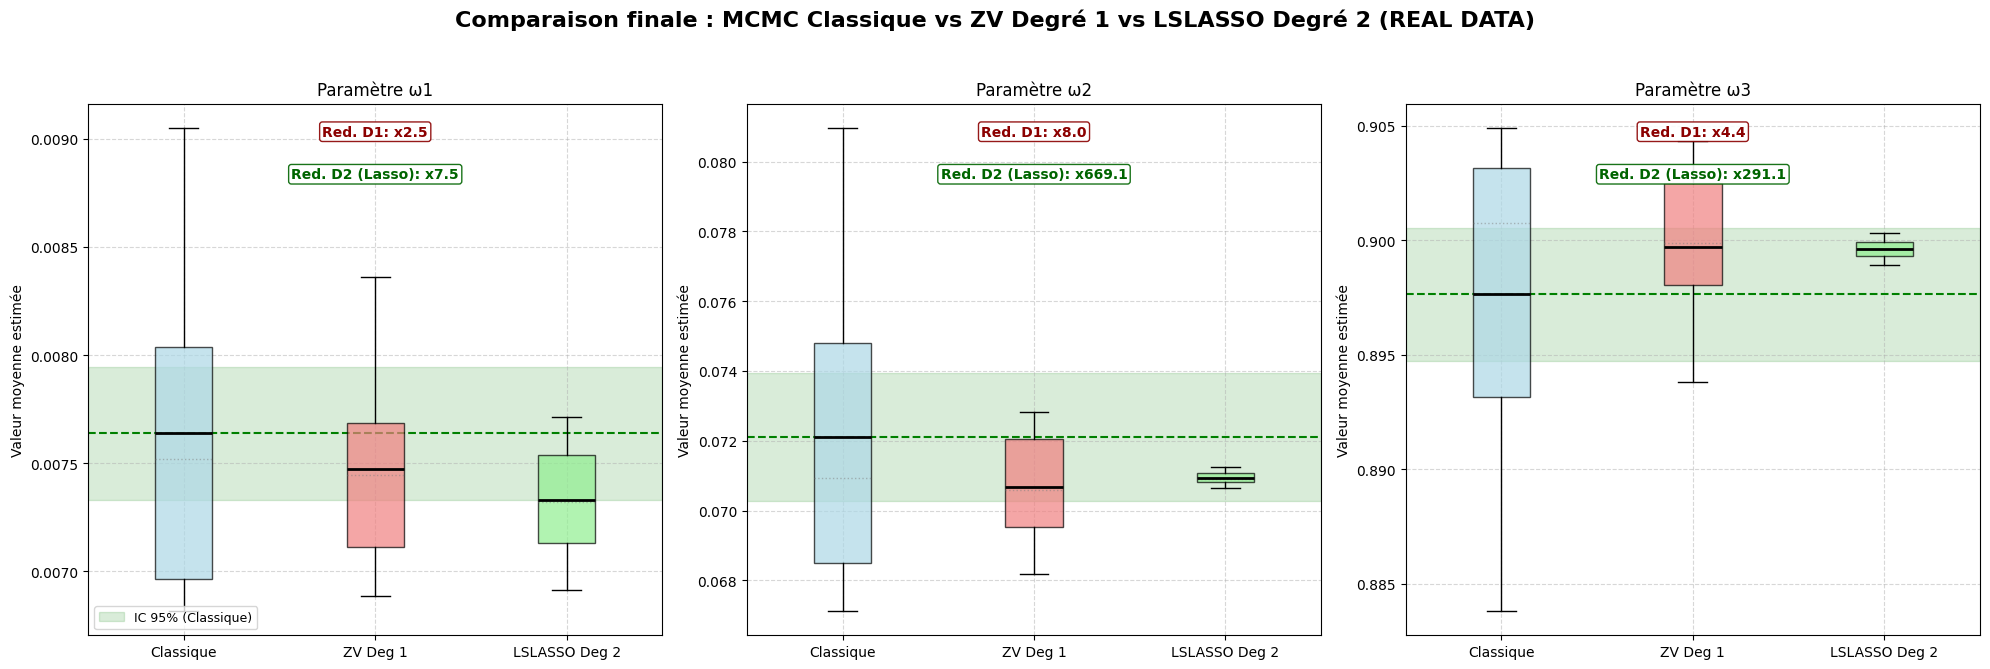
\includegraphics[width=\linewidth]{assets/notebook/q3_cell_31_out_00.png}
		\column{0.5\textwidth}
		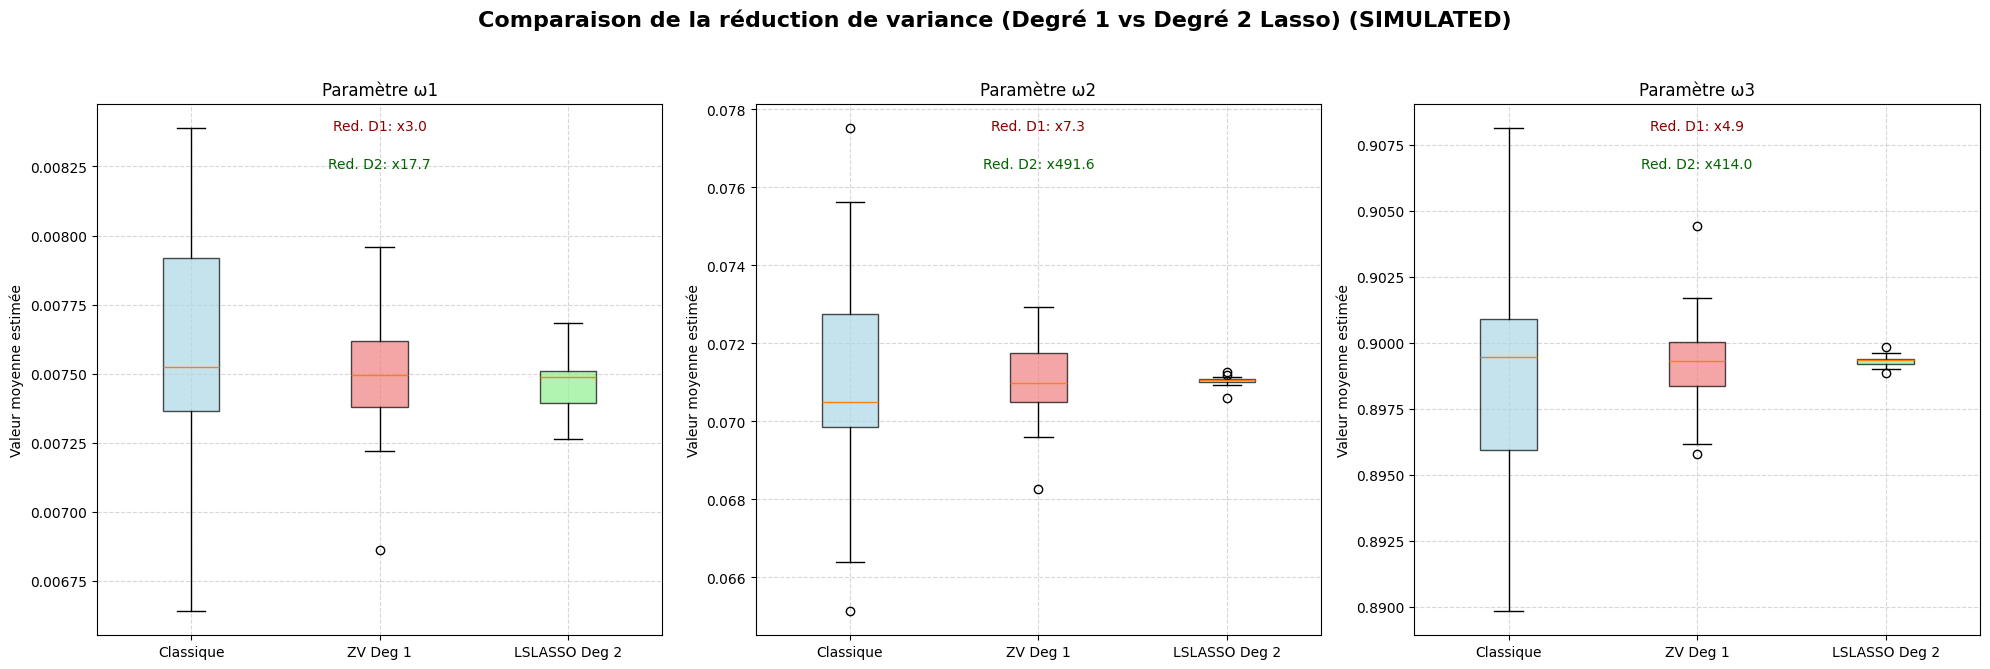
\includegraphics[width=\linewidth]{assets/notebook/q3_cell_32_out_00.png}
	\end{columns}
	\vspace{0.2em}
	\begin{itemize}
		\item LSLASSO remains competitive/improved when controls are many.
		\item Better bias-variance trade-off than one-shot OLS on large designs.
	\end{itemize}
\end{frame}

\begin{frame}{Part 4 -- Bonus Question}
	\Large
	\textbf{Is standard linear regression fully valid on MCMC draws?}\\[0.6em]
	Not exactly: draws are dependent.\\[0.3em]
	We tested practical fixes: \textbf{thinning} and \textbf{batching}.
\end{frame}

\begin{frame}{Q4 -- Dependence in MCMC (math view)}
	\small
	For a chain \((X_t)\), CLT involves integrated autocorrelation:
	\[
		\sqrt{N}\big(\bar f_N-\mu_f\big)\ \Rightarrow\
		\mathcal N(0,\sigma_f^2\tau_{\text{int}}),
	\]
	\[
		\tau_{\text{int}}=1+2\sum_{k\ge1}\rho_k.
	\]
	Effective sample size:
	\[
		\mathrm{ESS}\approx \frac{N}{\tau_{\text{int}}}.
	\]
	Practical fixes:
	\[
		\text{Thinning: }X'_m=X_{mk},
		\qquad
		\text{Batching: }B_m=\frac1b\sum_{t=(m-1)b+1}^{mb}X_t.
	\]
\end{frame}

\begin{frame}[fragile]{Q4 -- Dependence mitigation (code extract)}
	\begin{lstlisting}[style=py]
def apply_thinning(chain, k):
    return chain[::k]

def apply_batching(chain, batch_size):
    n_batches = len(chain) // batch_size
    truncated = chain[:n_batches * batch_size]
    return truncated.reshape(n_batches, batch_size, 3).mean(axis=1)
\end{lstlisting}
	\vspace{-0.5em}
	\begin{itemize}
		\item Thinning lowers autocorrelation by subsampling.
		\item Batching averages local dependence and approximates iid blocks.
	\end{itemize}
\end{frame}

\begin{frame}{Q4 -- Empirical comparison}
	\centering
	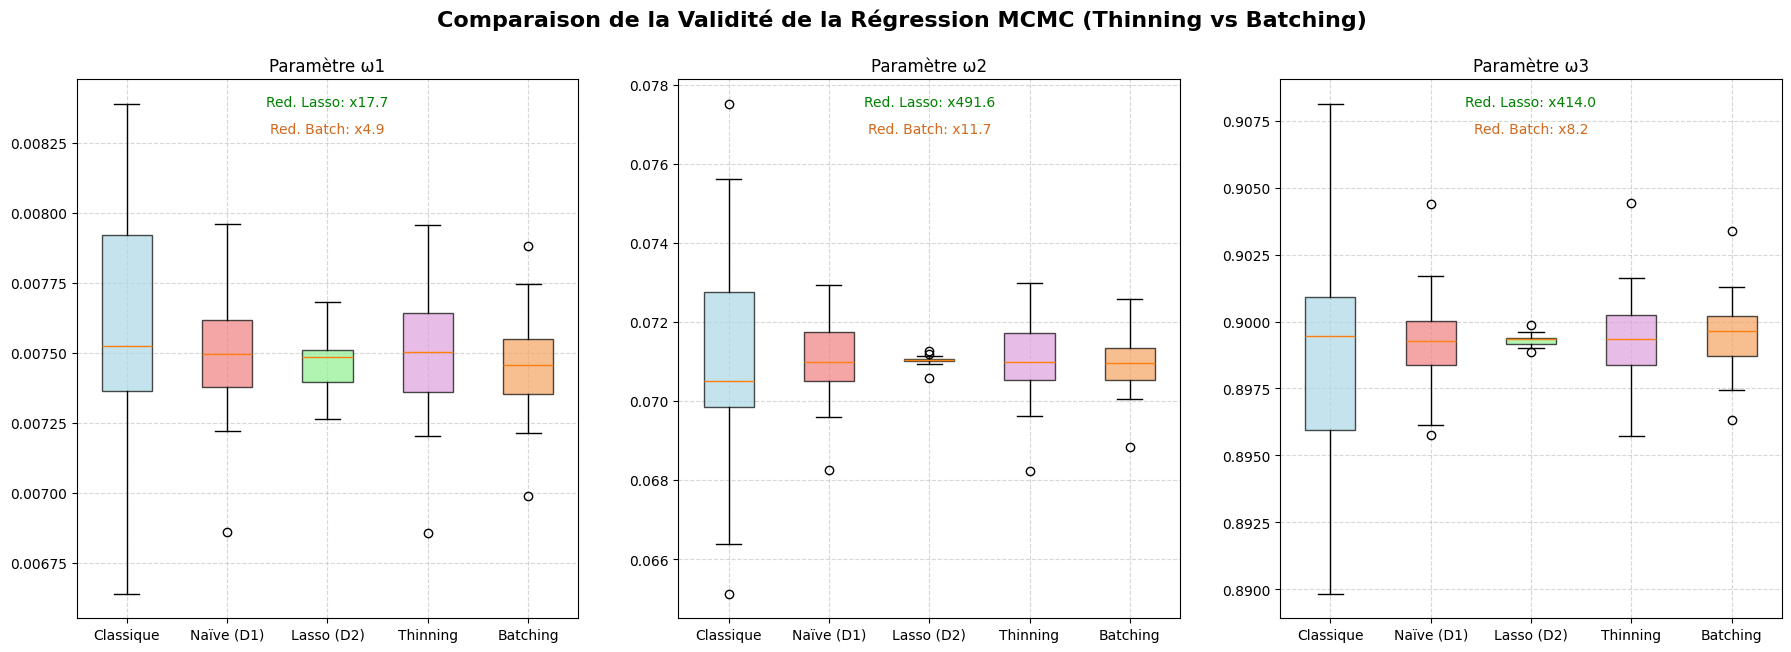
\includegraphics[width=0.82\linewidth]{assets/notebook/q4_cell_39_out_00.png}
	\begin{itemize}
		\item Dependence-aware variants can improve stability of corrections.
		\item Practical choice depends on ESS/cost trade-off.
	\end{itemize}
\end{frame}

\begin{frame}{Takeaways}
	\begin{itemize}
		\item RW-Metropolis works for simulated and real GARCH data.
		\item Control variates (degree 1) clearly reduce Monte Carlo error.
		\item Degree-2 controls become expensive; LSLASSO is a scalable fix.
		\item Bonus: accounting for MCMC dependence is important in practice.
	\end{itemize}
\end{frame}

\end{document}
